\section{Tachysséma Développement}
\subsection{Présentation de la Société}

\begin{figure}[ht]
    \centering
    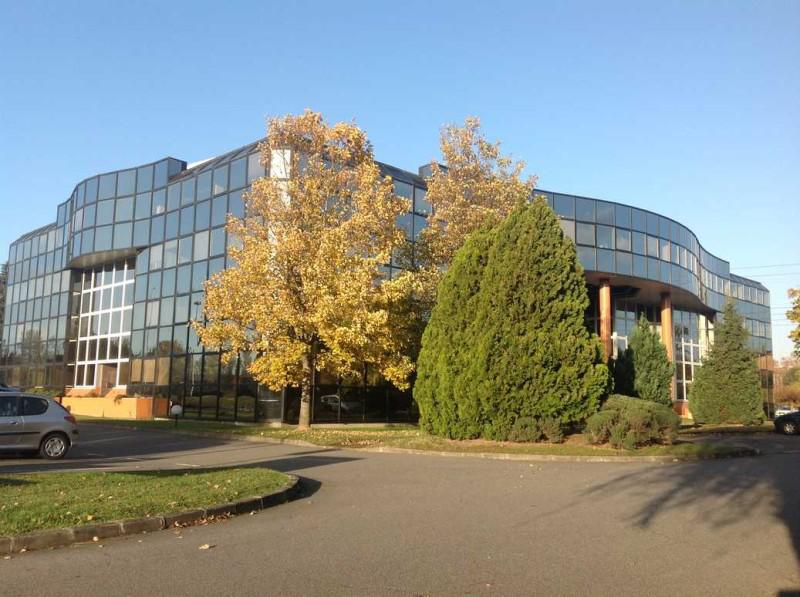
\includegraphics[scale=0.3]{img/bureau.jpg}
    \caption{Batiment Innopolis à Labège(31) où se situe Tachysséma Développement }
    \label{fig:CameraCmdsettings}
\end{figure}



Dans le cadre du master SME, je réalise ma première année d'alternance au sein de la SARL TACHYSSEMA DEVELOPPEMENT basée à Labège (31).
Cette société est impliquée dans des projets en lien avec le traitement vidéo et le traitment du signal en temps réel pour des systèmes éléctroniques embarqués. 

En conséquence, la société possède un rayon d'action étendu qui comprend de la R\&D, du développement matériel (caméras embarquées, conception de cartes éléctroniques) et du dévellopement logiciel. La société est notament spécialisée dans le développement de solutions basées la technologie FPGA.  

Les domaines d'applications de la société sont également variés puisque la société peut être amenée à réaliser des projets pour les secteurs de l'aéronautique, médical, militaire ou encore automobile. 



\subsection{Organisation interne}

Les locaux de Tachysséma Développement sont partagés avec Visif Technology, une société spécialisée dans le dévellopement de solutions technologiques pour les énergies renouvelables. Cependant les deux sociétés possèdes des projets communs et coopèrent ensembles sur ces projets. 

Au sein de Tachysséma Développement, Nicolas Roddier, mon tuteur d'alternance et gérant de la société est assité par un ingénieur automaticien ainsi qu'une stagiaire en M2 SME, un alternant en M2 SME et moi même. 





\newpage

\section{Projets Réalisés}
Dans cette partie nous réaliserons la synthèse des projets principaux menés depuis mon arrivée chez Tachysséma Développement, en septembre 2019. 

\subsection{Réalisation d'une IHM}

Dans le cadre d'un projet de gestion et contrôle des pixels deffectueux présents sur un capteur d'une caméra, j'ai réalisé une interface homme machine permettant d'établir un lien entre l'utilisateur et un module FPGA qui contrôle le capteur d'une caméra. 
\\ 

\subsubsection{Contexte} 

Le capteur d'une caméra est constitué d'un ensemble pixels qui captent la lumière entrante. On peut représenter l'ensemble de ces pixels sous la forme d'une matrice. Avec le temps, il est possible que certains pixels deviennent deffectueux, on parle alors de pixels morts. Les pixels deffectueux doivent pouvoir être localisés, corigés ou remplacés.  
\newline

La caméra est composée d'un FPGA qui contrôle le capteur vidéo. Il permet notament de réaliser le traitement des pixels deffectueux. L'interface homme machine interragit avec le FPGA, elle permettra la réalisation d'actions de lectures et d'écriture dans une table qui contient les coordonnées matricielle des pixels morts. 

\subsubsection{Cahier des charges de l'IHM } 

\begin{figure}[ht]
	\centering
    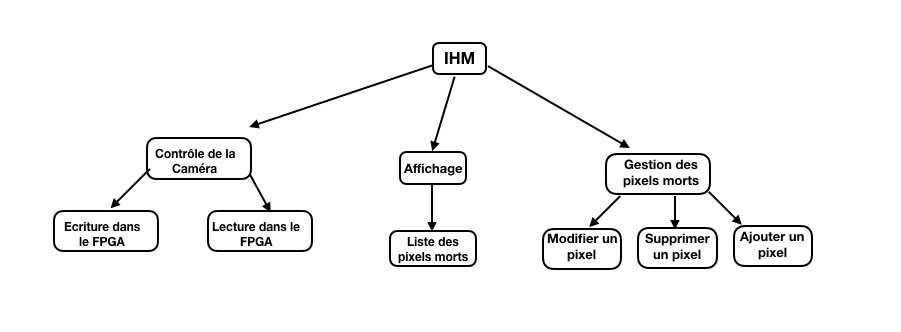
\includegraphics[scale=0.5]{img/cdcIHM.png}
    \caption{Cahier des charges de l'IHM}
    \label{fig:mavgen}
\end{figure}

Voici ci-dessous les principales fonctions qui sont réalisées par l'IHM : 
\newline
\begin{itemize}
	\item L'utilisateur peut lire et écrire la liste des pixels déffectueux dans un fichier .txt qui est sauvegardé sur le disque dur de l'ordinateur (où est executée l'IHM). 
	\item L'IHM peut intérragir avec la caméra par le biais d'une communication série. Elle réalise des opérations de lectures et d'écritures dans une table FPGA ainsi que dans une mémoire EEPROM qui contient les coordonnées des pixels défectueux. 
	\item Une fois que les coordonnées des pixels morts sont chargées de la caméra vers l'IHM ou du fichier .txt vers l'IHM, cette dernière les affiches sous la forme d'une liste comportant deux colonnes (une pour la ligne et une pour la colonne du pixel mort). 
	\item L'utilisateur peut effectuer différentes actions sur la liste des mauvais pixels. Il peut notament ajouter, supprimer ou remplacer des pixels deffectueux. A chaque modification, la liste est actualisée et transmise au FPGA.

\end{itemize}

\subsubsection{Implémentation}

\begin{figure}[ht]
    \centering
    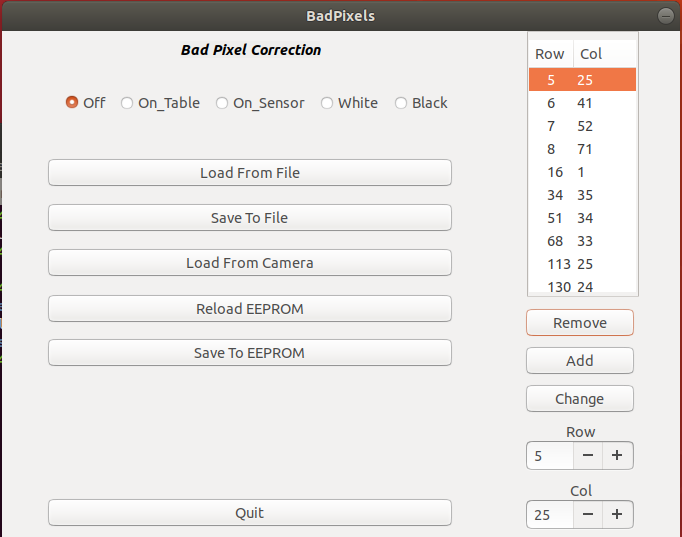
\includegraphics[scale=0.45]{img/IHM.png}
    \caption{Apperçu de l'IHM}
    \label{fig:CameraCmdsettings}
\end{figure}

\subsubsubsection{Interface graphique}

La première étape que j'ai effectué sur ce projet est la réalisation de la partie graphique de l'IHM. Cette dernière devait s'éxecuter sur une distribution linux.

En conséquence j'ai utilisé l'outil de développement graphique Glade qui intègre GTK+. Glade permet de faciliter la réalisation d'interfaces graphiques: En effet le développeur vient placer les différents objets ( boutons, champs de textes, curseurs etc .. ) sans passer par le code. 

Une fois ce processus terminé, glade génrère la solution obtenu dans un fichier .XML que nous pouvons intégrer directement dans un langage de programmation ( C, C++, Pyhton et d'autres encore). 
\newline

\subsubsubsection{Implémentation du code}

Ensuite j'ai pu implémenté le code en langage C qui permet d'établir un lien entre un évenement lié à l'interface graphique ( appuie sur un bouton, changement de valeur sur un curseur ..) et une fonction répondant au cahier des charges ( envoie des données dans le FPGA, quitter l'IHM ou encore écrire le fichier .txt par exemple). 



\subsection{Projet WindFloat Atlantic : Traitement des données d'un équipement embarqué}

\begin{figure}[ht]
    \centering
    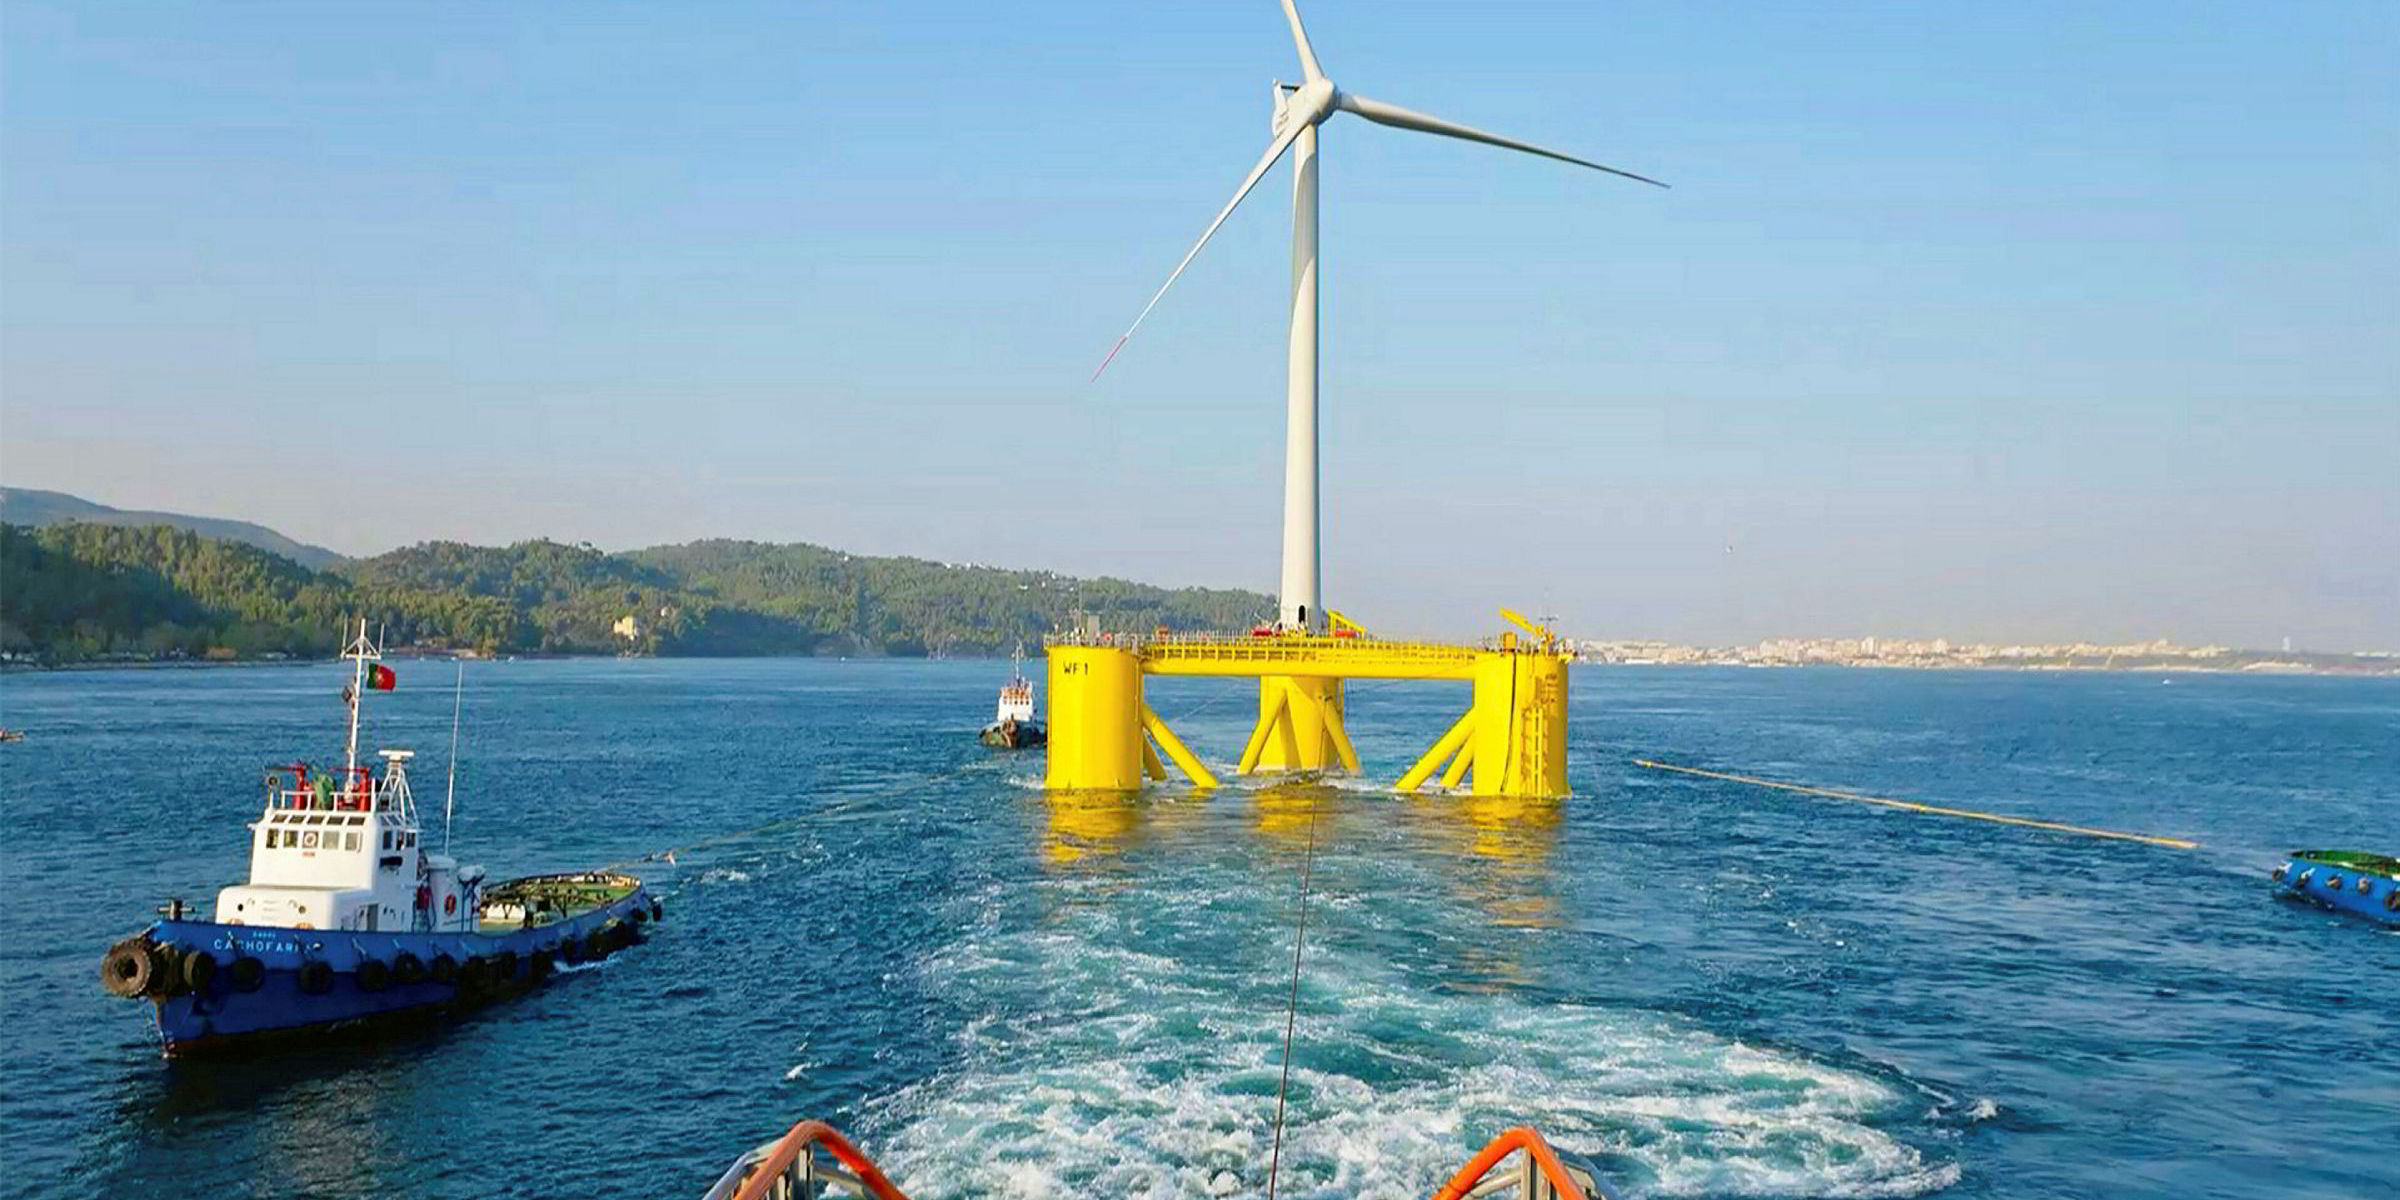
\includegraphics[scale=0.15]{img/WindFloatProject.jpeg}
    \caption{Plateforme située au Portugal}
    \label{fig:CameraCmdsettings}
\end{figure}

\subsubsection{Contexte}
\subsubsubsection{Le projet WindFloat Atlantic}

Tachyssema Developpement participe au projet WindFloat Atlantique mené par EDP Renewables, Engie, Repsol et Principle Power Inc. Ce projet de grande ampleur consite à la réalisation de plateformes exploitants l'énergie éolien offshore.

"WindFloat permet de développer des ressources énergétiques dans de vastes zones marines et de relever des défis majeurs, tels que la transition vers le zero carbone, la sécurité énergétique et la lutte contre le changement climatique, tout en créant des emplois, une croissance économique et des opportunités pour des investissements durables." (source : www.engie.com )

\subsubsubsection{Traitement des données utile pour l'asservissement d'une plateforme}
Informations utiles: Le Xsens MTi-10-series est un module qui regroupe un ensemble de capteurs permettant d'obtenir des informations d'une grande précision sur l'orientation, l'inclinaison, les accélérations sur 3 axes ( x,y,z) ainsi que les positions GPS. 
\newline

Les plateformes sont équipés d'un asservissement leurs permettants de rester stables malgrès des conditions métérologiques pouvant être difficiles comme dans le cas d'une forte houle ou de vents trop importants. Les plateformes sont équipés de trois flotteurs qui assurent leurs bon équilibre. Des pompes à eau sont présentes dans chaque flotteur. L'asservissement agit sur la commande de ces pompes à eau pour maintenir les plateformes en équilibre. 

Les positions GPS doivent aussi être connu en temps réel pour vérifier que les plateformes ne dérives pas. 
Toutes ces données proviennent de modules Xsens installés directement sur les plateformes qui transmettent les informations par communication série à un automate qui est lui même relié au sol via le protocole de communication MODBUS.  (voir figure ci-dessous)
\newpage


\begin{figure}[ht]
    \centering
    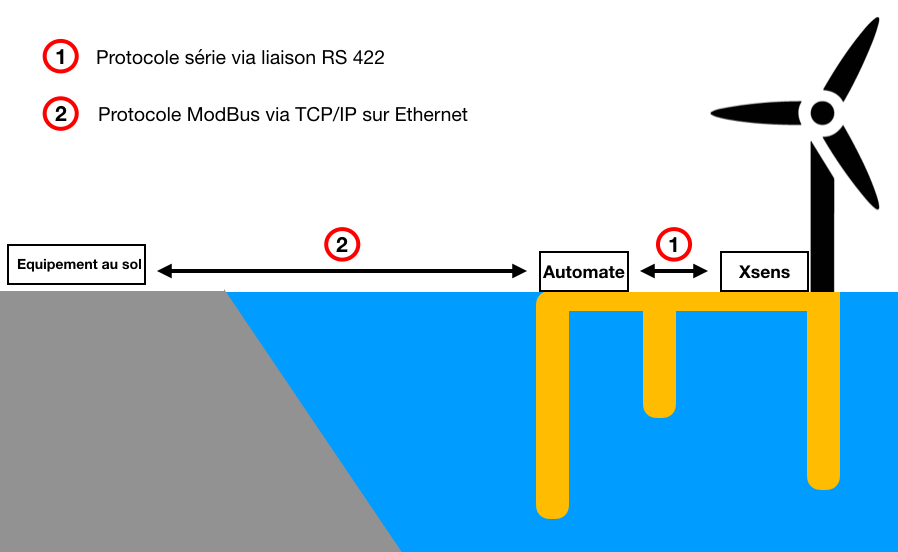
\includegraphics[scale=0.45]{img/schKOWL.png}
    \caption{Illustration de la communication entre équipements }
    \label{fig:CameraCmdsettings}
\end{figure}

\subsubsection{Travail effectué}

Ma mission sur ce projet consistait à : 

\begin{itemize}
	\item Configurer le module Xsens pour que les données répondants au cahier des charges soient transmises à la bonne fréquence (qui était initialement de 50 Hz). Les données utiles étaient donc le lacet (yaw), le roulis (roll), le tangage (pitch), la lattitude, la langitude ainsi que les accélérations X,Y et Z. 
	\item Etudier la trame générée par le module Xsens, le fonctionnement de la réception série de l'automate et la transmission des données en provenance de l'automate via le protocole MODBUS. 
	\item Créer un executable en C\# (s'exécutant sur un équipement au sol) permettant de lire les données disponibles sur l'automate, de les interpréter pour reconstituer la trame du module Xsens et enfin d'extraire les informations souhaitées. 

\end{itemize}
\newpage
\subsection{Etude du protocole MAVLINK }

\subsubsection{Présentation du protocole}

\begin{figure}[ht]
    \centering
    
\includegraphics[scale=0.45]{img/mavlink.png}
    \caption{Logo du protocole Mavlink }
    \label{fig:CameraCmdsettings}
\end{figure}

MAVLINK est un protocole qui permet de communiquer avec les drones (et entre les composants embarqués dans les drones). Un ensemble de messages Mavlink sont intégrés dans les librairies ce qui offre de larges possibilitées pour échanger des informations prédéfinies dans ces messages entre divers composants comme par exemple des servos moteurs, des capteurs, des modules GPS ou encore des caméras. 
\newline
On note que l'ensemble de ces messages sont définis dans un fichier .XML qui peut ensuite être généré dans un langage de programmation spécifique comme le C , le C++, le Python ou encore la JAVA pour les plus communs. En conséquence, ce protocole profite d'une grande portabilité. 

\subsubsection{Etude du protocole Mavlink pour l'intégration d'une Caméra }

Un client de Tachysséma Développement souhaiterait intégrer une caméra au sein d'un système utilisant le protocole Mavlink. Le cahier des charges précis du client n'étant pas encore définit, il me fallait donc étudier qu'elles étaient les possibilitées offertes par le protocole Mavlink pour l'intégration d'une caméra. 
\newline
Ma mission au sein de ce projet fut dans un premier temps l'étude des messages existants dans le protocole en rapport avec une caméra. Dans un second temps, dans le but d'ajouter des fonctionnalitées nouvelles non présentes dans le protocole, j'ai recherché quelles pouvaient être les solutions envisageables pour créer de nouveaux messages compatibles avec le protocole. 

\subsubsubsection{Echanges Mavlink natifs existants}

Le protocole Mavlink contient différents messages en rapport avec les caméras pouvant être utiles pour le client : 

\begin{itemize}
	\item Des messages pour effectuer des demandes de début de captures vidéos et arrêt de captures vidéos. 
	\item Des messages pour effectuer des demandes d'obtention des paramètres d'une caméra ( longueur de focal, nom du vendeur, firmware ...).
	\item Des messages pour configurer une caméra comme par exemple configurer le focus, le zoom etc ... 
\end{itemize}


\subsubsubsection{Implémentation d'un échange Mavlink}

Dans un deuxième temps et avec l'aide Pédro CARVALHO MENDES, alternant en deuxième année de master SME,  nous avons simmulé l'échange de messages Mavlink pour étudier le protocole. Voici un exemple d'échange que nous avons implémenté :  
\newpage
\begin{figure}[ht]
    \centering
    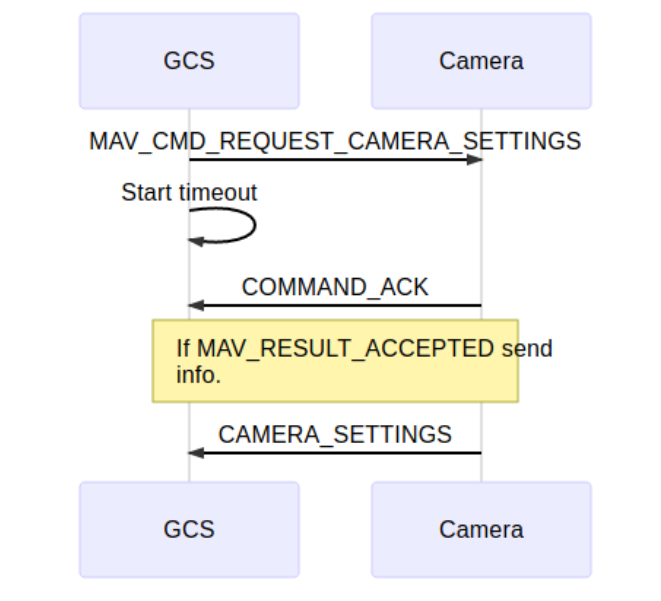
\includegraphics[scale=0.35]{img/mavlink_ech.png}
    \caption{Exemple d'échange Mavlink}
    \label{fig:CameraCmdsettings}
\end{figure}

avec GCS : Ground  Control Station

\subsubsubsection{Echanges Mavlink non-existants}

Dans le cas ou le client désirerait échanger des informations non incluses dans des messages Mavlink existants comme par exemple le numéro de série d'une caméra ou des paramètres spécifiques, nous avons du trouver une méthode permettant d'ajouter des messages personnalisés au protocole Mavlink. 
\newline

Pour ce faire nous avons créé un nouveau fichier .XML qui contient la définition des nouveaux messages. Ce fichier est ensuite généré (grâce au générateur Mavlink) dans le langage de programmation voulu et peut être intégré à la bibliothèque Mavlink. 



\begin{figure}[ht]
    \centering
    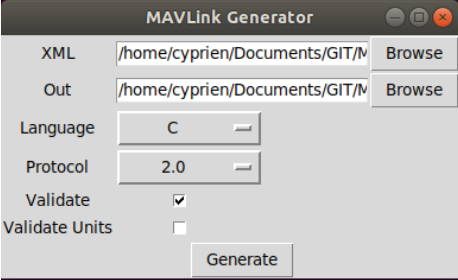
\includegraphics[scale=0.6]{img/mavlink_gen.png}
    \caption{Générateur Mavlink}
    \label{fig:CameraCmdsettings}
\end{figure}
